%%%% utfprpgtex-article.tex, 2019/02/20
%%%% Copyright (C) 2016-2019 Luiz E. M. Lima (luizeduardomlima@gmail.com)
%%
%% Este arquivo pode ser distribuído e/ou modificado sob as condições da
%% Licença Pública do Projeto LaTeX, tanto a versão 1.3 desta licença ou (à sua
%% opção) qualquer versão posterior.
%% A versão mais recente desta licença está disponível em
%%   http://www.latex-project.org/lppl.txt
%% e a versão 1.3 ou posterior faz parte de todas as distribuições de LaTeX
%% versão 2005/12/01 ou posterior.
%%
%% Este arquivo tem o estado de manutenção da LPPL `mantida'.
%%
%% O mantenedor atual deste arquivo é Luiz E. M. Lima.
%%
%% Este projeto consiste dos arquivos utfprpgtex-article.sty e
%% utfprpgtex-article.tex.
%%
%% utfprpgtex-article.tex é o arquivo principal do modelo LaTeX (não oficial)
%% para produção de artigo da Universidade Tecnológica Federal do Paraná
%% (UTFPR). Foi desenvolvido baseado no modelo de artigo do abnTeX2, disponível
%% em <http://www.abntex.net.br/>.

%% Passagem de opções para pacotes
\PassOptionsToPackage{english, main = brazilian}{babel}%% Suporte multilíngue

%% Classe e opções de documento
\documentclass[%% Opções
%%%% Opções da classe memoir
  article,%% Tipo de documento: article, book, report, etc.
  10pt,%% Tamanho de fonte: 10pt, 11pt, 12pt, etc.
  a4paper,%% Tamanho de papel: a4paper, letterpaper, etc.
  fleqn,%% Alinhamento de equações à esquerda (comente para centralizado)
  oneside,%% Impressão de elementos textuais e pós-textuais: oneside (anverso) ou twoside (anverso e verso)
  % twocolumn,%% Impressão em duas colunas (comente para uma coluna)
%%%% Opções da classe abntex2
  sumario = tradicional,%% Estilo de sumário: tradicional (padrão) ou abnt-6027-2012 (ABNT NBR 6027-2012)
  chapter = TITLE,%% Títulos de capítulos em maiúsculas (comente para desabilitar)
  section = TITLE,%% Títulos de seções secundárias em maiúsculas (comente para desabilitar)
  % subsection = TITLE,%% Títulos de seções terciárias em maiúsculas (comente para desabilitar)
  % subsubsection = TITLE,%% Títulos de seções quartenárias em maiúsculas (comente para desabilitar)
]{abntex2}

%% Pacotes utilizados
\usepackage{utfprpgtex-article}%% Estilos do modelo
\usepackage{lipsum}%% Geração de texto fictício

%% Arquivo de referências
\addbibresource{utfprpgtex-article.bib}

%% Informações do documento
\titulo{%% Título
  TÍTULO DO TRABALHO ACADÊMICO (ARTIGO OU PROJETO)%
}
\tituloemoutroidioma{%% Título em outro idioma
  TITLE OF ACADEMIC WORK (ARTICLE OR PROJECT)%
}
\autor{%% Autor(es) e e-mail(s)
  Primeiro(a) Autor(a)\thanks{\email{autor1@dominio}, Curso de <Nome do Curso>.}\\%
  Segundo(a) Autor(a)\thanks{\email{autor2@dominio}, Curso de <Nome do Curso>.}\\%
  Terceiro(a) Autor(a)\thanks{\email{autor3@dominio}, Curso de <Nome do Curso>.}%
}
\instituicao{\utfprname}%% Instituição --- Automático
\campus{PG}{Câmpus Ponta Grossa}%% Câmpus: {sigla} e {nome}
\departamento[logo-da]{<DEPTO>}{%% Depto., Coord., Prog. ou Curso: [logo], {sigla} e {nome}
  Departamento Acadêmico de <Nome do Depto.>%
}
\local{Ponta Grossa, Paraná, Brasil}%% Local
\data{}%% Data --- Comente para gerar a data atual

%% Ferramenta para criação de índices
\makeindex

%% Início do documento
\begin{document}

\pretextual%% Elementos pré-textuais

\begin{paginadetitulo}%% Página de título

\begin{ambienteresumo}%% Resumo
O texto do resumo deve situar o trabalho no contexto geral e a importância do tema estudado, descrever de forma breve os objetivos, a metodologia adotada, os resultados obtidos e as principais conclusões, relatando a contribuição própria, em não mais de 250 palavras. Não deve conter nem fórmulas ou deduções matemáticas e nem citações bibliográficas.
\palavraschave{palavra 1. palavra 2. palavra 3\dots{} (no máximo 5).}%% Palavras-chave
\end{ambienteresumo}

\begin{ambienteresumo}[Abstract]%% Abstract
\begin{otherlanguage*}{english}%% Idioma do abstract
The abstract text should place the work in the general context and the importance of the topic studied, briefly describe the objectives, the methodology adopted, the results obtained and the main conclusions, reporting the own contribution, in no more than 250 words. It should contain neither mathematical formulas nor deductions nor bibliographical citations.
\palavraschave[Keywords]{word 1. word 2. word 3\dots{} (maximum 5).}%% Keywords
\end{otherlanguage*}
\end{ambienteresumo}

\end{paginadetitulo}

\textual%% Elementos textuais

\section{Introdução}\label{sec:intro}

O texto desta seção deve contextualizar o tema a ser analisado e/ou desenvolvido no trabalho, definindo o problema e sua importância, apresentando uma breve revisão teórica e/ou bibliográfica\footnote{As referências podem ser encontradas em <\url{http://www.periodicos.capes.gov.br/}> e/ou <\url{http://scholar.google.com.br/}>.} (breve descrição dos trabalhos mais relevantes que estão relacionados ao tema apresentando suas principais contribuições) e, finalmente, apresentando as considerações adotadas e objetivos (contribuições referentes ao trabalho proposto com base na revisão da literatura apresentada).

\section{Metodologia}\label{sec:met}

O texto desta seção deve apresentar o desenvolvimento do tema, descrevendo o(s) método(s) de análise (teórico e/ou experimental) utilizado(s) para a obtenção dos resultados no desenvolvimento da pesquisa para que a mesma possa ser reconstituída.

\subsection{Teórica}\label{ssec:teor}

A metodologia teórica (analítico e/ou numérico) deve apresentar: a descrição, a configuração e as hipóteses do problema (permanente ou transiente; 1D, 2D ou 3D; etc.); as equações governantes, as condições de contorno e os modelos utilizados (apresentar referências da literatura para equações e modelos, quando pertinente); o método de solução e a malha computacional (descrever programas e/ou ferramentas utilizadas e/ou códigos desenvolvidos); o método de análise e/ou comparação dos resultados (desvios absolutos e/ou relativos; RMS; etc.).

\subsection{Experimental}\label{ssec:exp}

A metodologia experimental deve apresentar: a descrição do aparato experimental (desenhos esquemáticos; fotos; etc.); a descrição do(s) instrumento(s) de medição (faixa(s) de operação e incerteza(s)); descrição do(s) procedimento(s) para execução do experimento, de medição e dos cálculos necessários.

\section{Resultados}\label{sec:res}

O texto desta seção deve descrever detalhadamente os dados e/ou resultados obtidos pelo autor, que normalmente são apresentados na forma de quadros, tabelas, gráficos, etc. Deve ser efetuada a comparação dos dados obtidos e/ou resultados, com aqueles descritos na revisão de literatura, incluindo os comentários sobre os estudos de outros autores.

\section{Conclusões}\label{sec:concl}

O texto desta seção deve apresentar as conclusões do trabalho baseando-se nos resultados obtidos para mostrar a sua viabilidade técnica e/ou econômica. Deve finalizar o trabalho com uma resposta às hipóteses especificadas na introdução. O autor deve manifestar seu ponto de vista sobre os resultados obtidos; não se deve incluir novos dados ou equações. A partir da tese, alguns assuntos que foram identificados como importantes para serem explorados poderão ser sugeridos como temas para novas pesquisas.

\section{Informações sobre o Desenvolvimento do Projeto}\label{sec:infoproj}

Nesta seção, são apresentadas informações referentes ao desenvolvimento do projeto. Portanto, esta seção não deve fazer parte da versão final do projeto.

O projeto consiste na \textcolor{red}{proposição e realização de estudo} de alguma aplicação dos conceitos desenvolvidos na disciplina, principalmente os relacionados ao \textcolor{red}{nome do tema}, em algum dispositivo ou situação de interesse prático. Este estudo pode apresentar soluções analíticas, computacionais e/ou experimentais. O projeto é uma atividade \textcolor{red}{opcional}, pode ser desenvolvido \textcolor{red}{em grupo} (máximo 3 membros) e deve ser rigorosamente apresentado de acordo com estas instruções em duas etapas.

A \textcolor{red}{primeira etapa} consiste da entrega de uma \textcolor{red}{proposta de pesquisa} até data definida. Esta proposta deve apresentar informações até a introdução, bem como as referências, conforme este modelo. Esta etapa é uma pré-avaliação e, portanto, sujeita à aprovação do tema definido. A \textcolor{red}{segunda etapa} consiste da entrega do \textcolor{red}{projeto de pesquisa} até data definida. Este projeto de pesquisa deve apresentar informações de todas as seções deste modelo.

\section{Informações sobre a Formatação do Texto}\label{sec:infoform}

Nesta seção, são apresentadas informações referentes à formatação do texto. Portanto, esta seção não deve fazer parte da versão final do projeto. O texto do projeto deve ser rigorosamente formatado de acordo com estas instruções.

O arquivo de texto deste projeto está limitado a um máximo de 10 páginas, incluindo tabelas e figuras. O arquivo final em formato pdf (\textcolor{red}{Código}-Projeto-\textcolor{red}{Nome\_do\_Aluno}.pdf) não deve exceder 5 MB e pode ser gerado a partir do arquivo em formato do Microsoft Word (Modelo do Projeto.docx) ou a partir do editor online para LaTeX (disponível em <\url{http://www.papeeria.com/p/ca8c4367f7c9433b11307a3f720271f8?withLastOpenedFile=false}>). Para gerar a versão final a partir do arquivo do Microsoft Word lembre-se de mudar na guia revisão de ``Final: Mostrar Marcação'' para ``Final''.

O projeto deve ser digitado em papel tamanho A4, usando Fonte Times New Roman, tamanho 10, exceto para o título, nome e e-mail de autores, instituição, resumo e palavras-chave, que têm formatações específicas. Espaço simples entre linhas deve ser usado ao longo do texto. Todas as margens devem ter 2 cm, exceto a superior (2,5 cm).

\subsection{Títulos e Subtítulos das Seções}\label{ssec:tit}

Os títulos das seções e subseções devem ser digitados em formato Times New Roman, tamanho 10, negrito e alinhado à esquerda. Os títulos das seções devem ser formatados em letras maiúsculas (exemplo: \textbf{MODELO MATEMÁTICO}), enquanto que os títulos das subseções devem ter somente as primeiras letras em maiúsculas (exemplo: \textbf{Modelo Matemático}). Eles devem ser numerados, usando numerais arábicos separados por pontos, até o máximo de 3 subníveis. Uma linha em branco de espaçamento simples deve ser incluída acima e abaixo de cada seção/subseção.

\subsection{Corpo do Texto}\label{ssec:corpo}

O corpo do texto deve ser justificado e com espaçamento simples. A primeira linha de cada parágrafo deve ter recuo de 0,6 cm a partir da margem esquerda.

\subsubsection{Equações}\label{sssec:eqs}

As equações matemáticas devem ser alinhadas à esquerda com recuo de 0,6 cm (mas também podem ser centralizadas). As equações devem ser referenciadas por Eq.~\eqref{eq:Uxy} no meio da frase, ou por Equação~\eqref{eq:Uxy} quando usada no início de uma sentença. Os números das equações devem ser formatados com numerais arábicos colocados entre parênteses, e alinhados à direita, como mostrado na Eq.~\eqref{eq:Txy}. Os símbolos usados nas equações devem ser definidos imediatamente antes ou depois de sua primeira ocorrência no texto do trabalho. O tamanho da fonte usado nas equações deve ser compatível com o utilizado no texto. Todos os símbolos devem ter suas unidades expressas no Sistema Internacional (SI).

\begin{equation}\label{eq:Uxy}
\frac{\partial^2 U}{\partial x^2} + \frac{\partial^2 U}{\partial y^2} = 0
\end{equation}

\begin{equation}\label{eq:Txy}
\frac{\partial^2 T}{\partial x^2} + \frac{\partial^2 T}{\partial y^2} = 0
\end{equation}

Equações podem ser inseridas neste documento usando o ambiente \LaTeX\ ``equation'', conforme exemplo no arquivo fonte deste modelo. Símbolos matemáticos (ou equações mais simples) podem ser inseridos ao longo do texto de um parágrafo usando o ambiente \LaTeX\ ``math'' (\verb|$...$|), por exemplo: $\alpha$, $A = \pi D^{2} /4$, etc. Para gerar ou editar equações em \LaTeX\ pode-se utilizar a ferramenta ``Formula Sheet'', disponível em <\url{http://formulasheet.com/}>, dentre outras.

\subsubsection{Figuras}\label{sssec:figs}

As figuras devem ser centralizadas e referenciadas por Fig.~\ref{fig:grafico} no meio da frase ou por Figura~\ref{fig:grafico} quando usada no início de uma sentença. Sua legenda deve ser centralizada e localizada imediatamente acima da figura. As anotações e numerações devem tem tamanhos compatíveis com o da fonte usada no texto, e todas as unidades devem ser expressas no Sistema Internacional (SI). As figuras devem ser colocadas o mais próximo possível de sua primeira citação no texto. Deixe uma linha em branco entre as figuras e o texto.

\begin{figure}[!htb]
\centering
\caption{Comparação entre os resultados do presente modelo com os resultados experimentais de Wirtz e Stutzman (1982), em termos da diferença de temperatura em função da altura do canal.}
\label{fig:grafico}
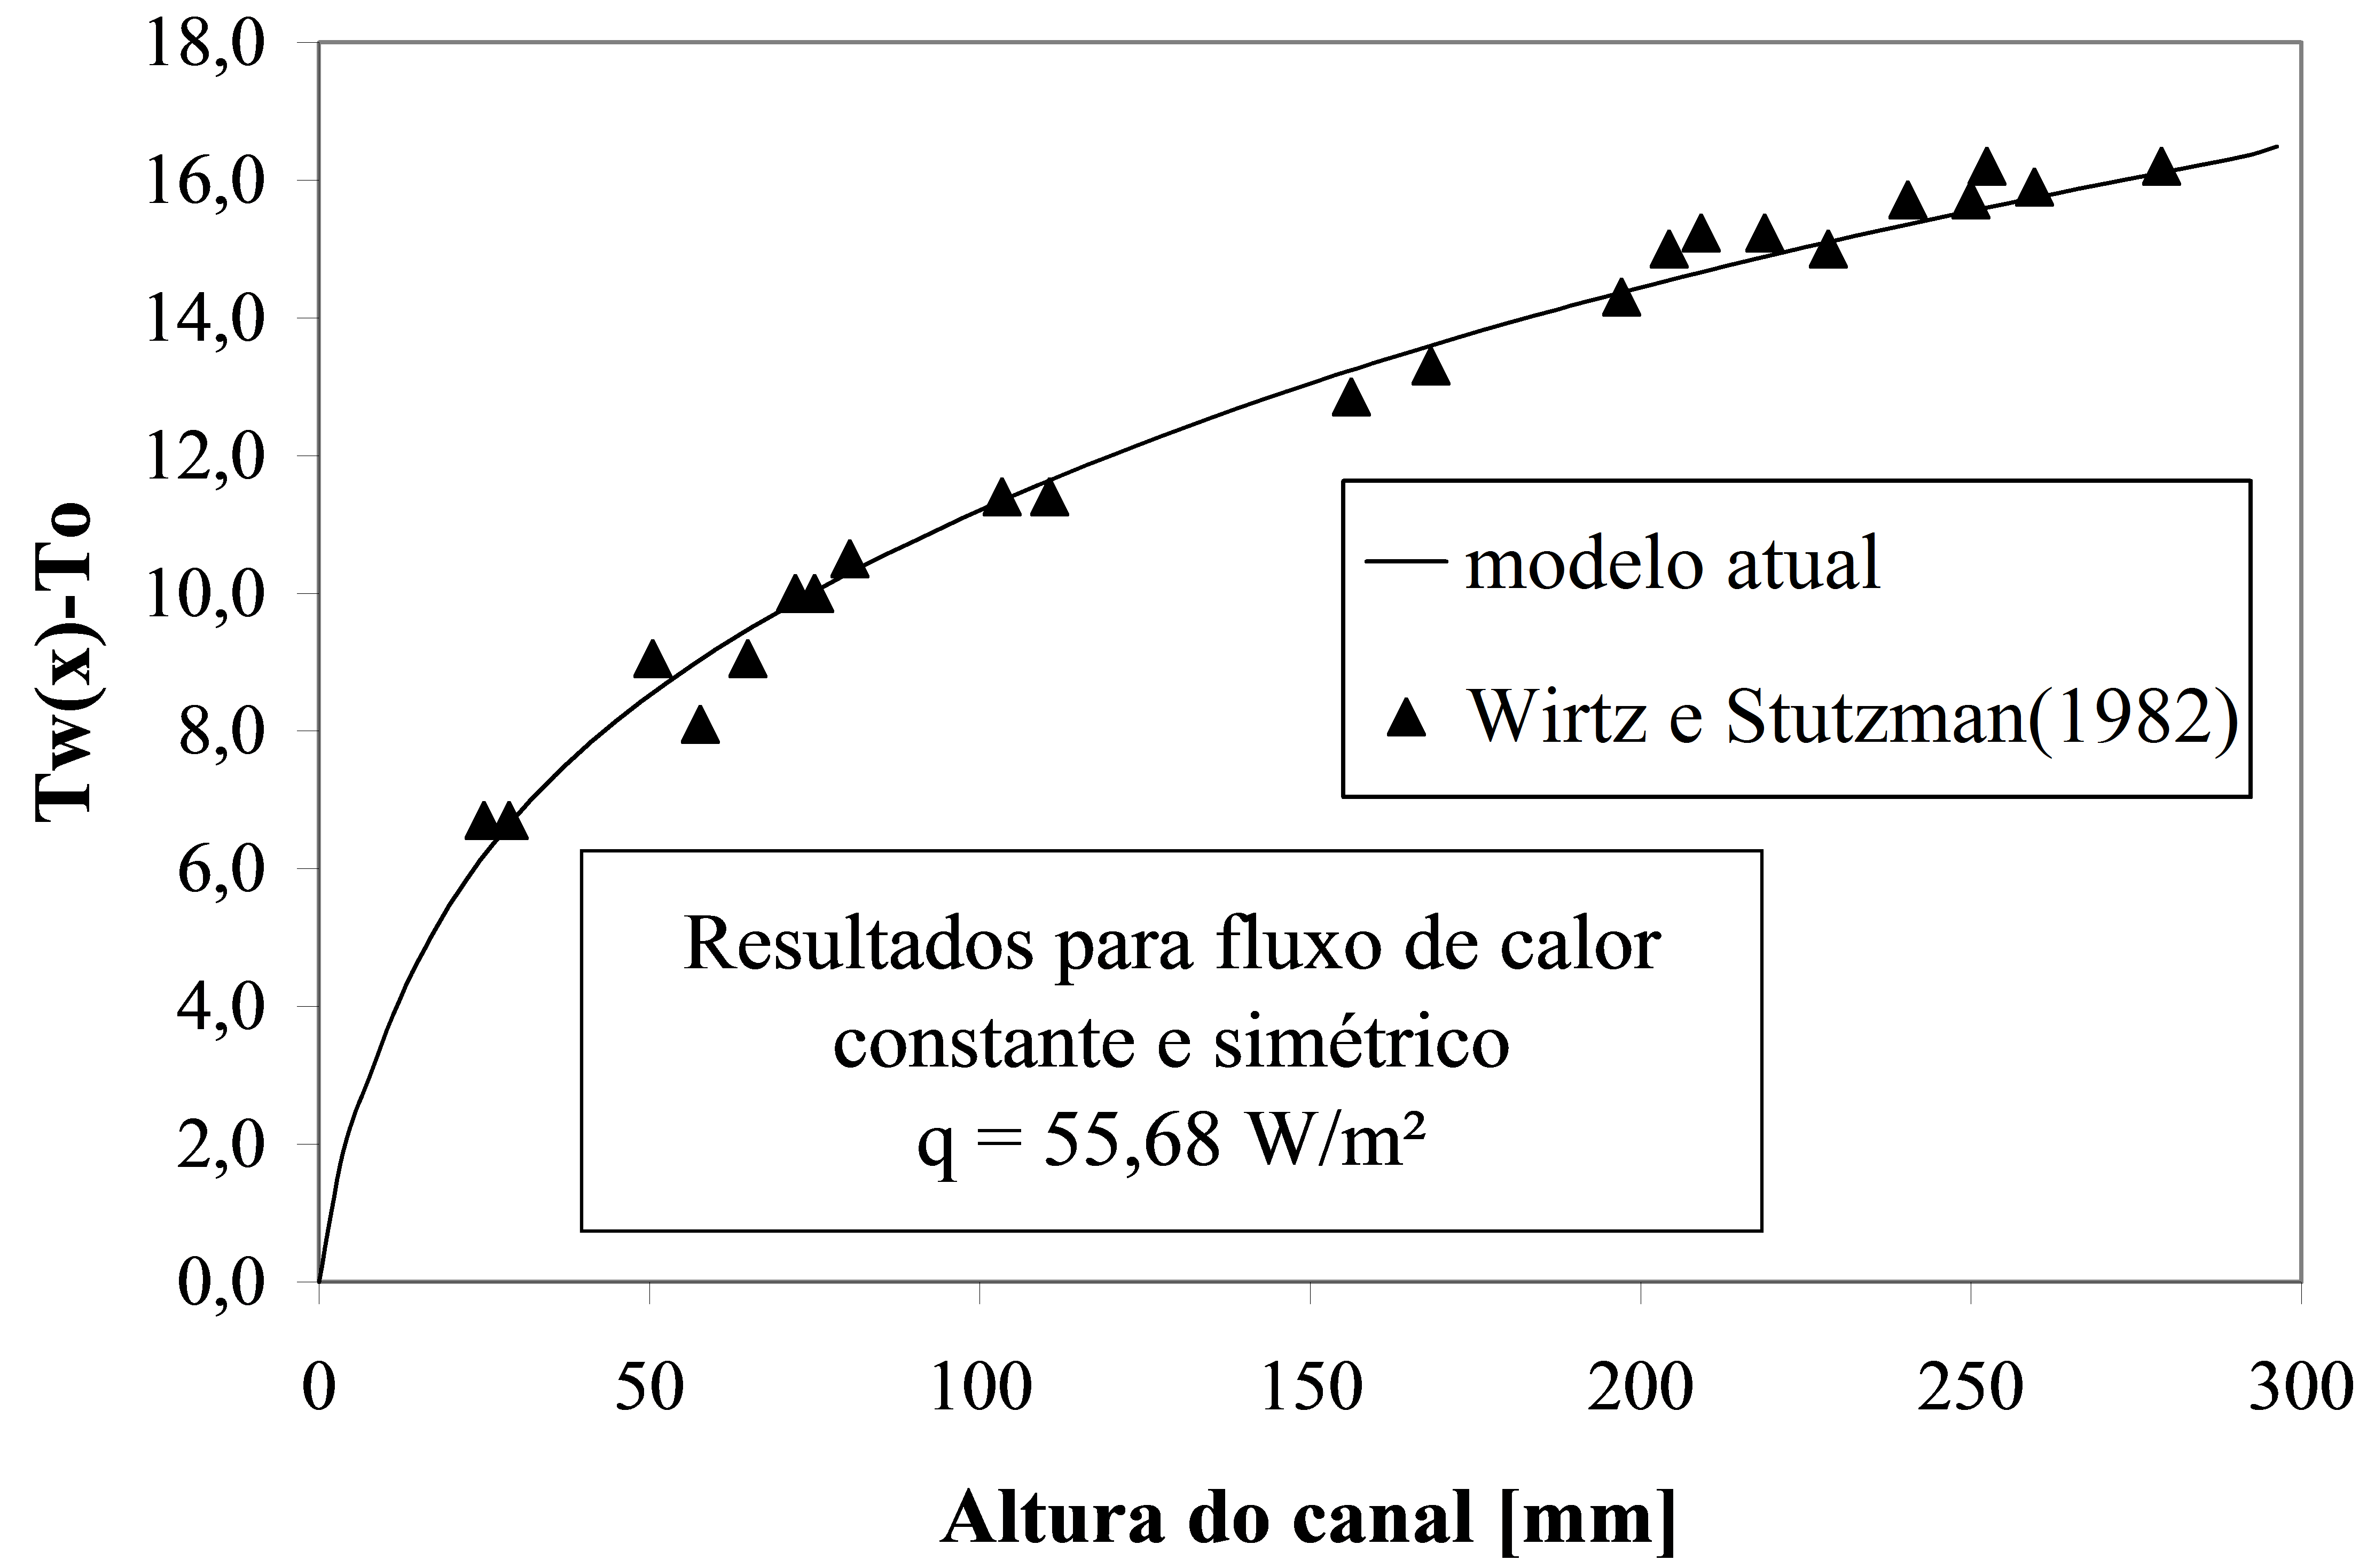
\includegraphics[width = 0.5\columnwidth]{./Figuras/grafico}
\fonte{Autoria própria.}
\end{figure}

Figuras coloridas e fotografias de alta qualidade podem ser incluídas no trabalho. Para reduzir o tamanho do arquivo e preservar a resolução gráfica, converta os arquivos das imagens para o formato GIF (para figuras com até 16 cores) ou para o formato JPEG (alta densidade de cores), antes de inseri-los no trabalho.

Figuras podem ser inseridas neste documento usando o ambiente \LaTeX\ ``figure'', conforme exemplo no arquivo fonte deste modelo.

\subsubsection{Tabelas}\label{sssec:tabs}

As tabelas devem ser centralizadas e referenciadas por Tab.~\ref{tab:resexp} no meio da frase, ou por Tabela~\ref{tab:resexp} quando usada no início de uma sentença. Sua legenda deve ser centralizada e localizada imediatamente acima da tabela. Anotações e valores numéricos nela incluídos devem ter tamanhos compatíveis com o da fonte usado no texto do trabalho, e todas as unidades devem ser expressas no Sistema Internacional (SI). As unidades devem ser incluídas apenas na primeira linha ou primeira coluna de cada tabela, conforme for apropriado. As tabelas devem ser colocadas tão perto quanto possível de sua primeira citação no texto. Deixe uma linha simples em branco entre a tabela, seu título e o texto. O estilo de borda da tabela é livre. As legendas das figuras e das tabelas não devem exceder 3 linhas.

\begin{table*}[!htb]
\centering
\caption{Resultados experimentais para as propriedades de flexão dos materiais CFRC-TWILL e CFRC-4HS. Valores médios obtidos em 20 ensaios.}
\label{tab:resexp}
\begin{tabular*}{\textwidth}{@{\extracolsep{\fill}}lll}
\hline
Propriedades do compósito    & CFRC-TWILL    & CFRC-4HS     \\ \hline
Resistência à Flexão / [MPa] & 209$\pm$10    & 180$\pm$15   \\
Módulo de Flexão / [GPa]     & 57,0$\pm$2,8  & 18,0$\pm$1,3 \\ \hline
\end{tabular*}
\fonte{Autoria própria.}
\end{table*}

Tabelas podem ser inseridas neste documento usando o ambiente \LaTeX\ ``table'', conforme exemplo no arquivo fonte deste modelo. Para gerar ou editar tabelas em \LaTeX\ pode-se utilizar a ferramenta ``Tables Generator'', disponível em <\url{http://www.tablesgenerator.com/}>, dentre outras.

\subsubsection{Citações e Referências}\label{sssec:citref}

As citações das referências no corpo do texto podem ser feitas no formato autor-ano da Associação Brasileira de Normas Técnicas (ABNT):

\begin{itemize}
\item Implícitas:
\begin{itemize}
\item ... \cite{VanEkenstein1997}.
\item ... \cite{Coleman1991,Nriagu1988}.
\item ... \cite{Wizentier1992,Faina2000,Larsson2018}.
\item ... \cite{VanEkenstein1997,Nriagu1988,Faina2000}.
\end{itemize}
\item Explícitas:
\begin{itemize}
\item \textcite{VanEkenstein1997} afirmam que...
\item ..., conforme visto em \textcite{Coleman1991,Nriagu1988}.
\item Segundo \textcite{Wizentier1992,Faina2000,Larsson2018},...
\item ... como as definições de \textcite{VanEkenstein1997,Nriagu1988,Faina2000}.
\end{itemize}
\end{itemize}

Referências aceitas incluem: artigos (de periódicos ou de anais de congressos), dissertações, teses, livros, comunicações privadas, etc. A lista de referências deve ser uma nova seção denominada Referências. Todas as referências incluídas na lista devem aparecer como citações no texto do trabalho. As referências devem ser postas em ordem alfabética, usando o último nome do primeiro autor. Um exemplo de lista de referências é apresentado na sequência.

Citações e referências podem ser inseridas neste documento usando os comandos do pacote \LaTeX\ ``biblatex'', disponível em <\url{http://ctan.org/pkg/biblatex/}>, conforme exemplos no arquivo fonte deste modelo. Os dados de cada referência podem ser obtidos de um arquivo ``bibtex'' (*.bib), geralmente na própria página de \textit{download} da referência (artigos, livros, etc.) ou, ainda, a partir do Google Acadêmico, etc. Para gerar ou editar entradas de arquivos ``bibtex'' (*.bib) pode-se utilizar a ferramenta ``Bibtex Editor'', disponível em <\url{http://truben.no/latex/bibtex/}>, ou ``ZoteroBib'', disponível em <\url{http://zbib.org/}>, dentre outras.

\subsubsection{Plágio Acadêmico}\label{sssec:plagio}

As devidas citações de referências para textos, figuras, tabelas, etc., bem como a apresentação de suas respectivas fontes de referência, são de extrema importância na redação de qualquer texto, principalmente acadêmico/científico, para que não se caracterize a prática de plágio.

A violação dos direitos autorais é CRIME previsto no Artigo 184 do Código Penal, com punição que vai desde o pagamento de multa até a reclusão de quatro anos, dependendo da extensão e da forma como o direito do autor foi violado. Além das penalidades citadas e da desmoralização acadêmica, o plagiário estará sujeito a sanções cíveis, como retratação pública e indenização pecuniária por dano moral e/ou patrimonial, e também a sanções administrativas, que podem chegar à reprovação/desligamento da instituição, no caso de estudantes, e demissão, no caso de professores/pesquisadores.

\subsection{Informações e Dicas sobre \TeX/\LaTeX}\label{ssec:texlatex}

\begin{itemize}
\item \LaTeX\ Project: <\url{http://www.latex-project.org/}>.
\item Comprehensive \TeX\ Archive Network (CTAN): <\url{http://www.ctan.org/}>.
\item \TeX\ Users Group (TUG): <\url{http://www.tug.org/}>.
\item \LaTeX\ - Wikibooks: <\url{http://en.wikibooks.org/wiki/LaTeX/}>.
\item \TeX\ - \LaTeX\ Stack Exchange: <\url{http://tex.stackexchange.com/}>.
\end{itemize}

\postextual%% Elementos pós-textuais

\printbibliography%% Referências

\begin{ambienteapendices}%% Apêndices

\chapter{Título do Apêndice}\label{cap:apendicea}

\lipsum[11-15]

\end{ambienteapendices}

\begin{ambienteanexos}%% Anexos

\chapter{Título do Anexo}\label{cap:anexoa}

\lipsum[21-25]

\end{ambienteanexos}

\chapter*{Agradecimentos}

O(s) autor(es) agradece(m) à Universidade Tecnológica Federal do Paraná pelo apoio recebido para o desenvolvimento do presente trabalho.

\chapter*{Declaração de Responsabilidade}

O(s) autor(es) é(são) o(s) único(s) responsável(eis) pelo material impresso contido neste documento.

%% Fim do documento
\end{document}
